\documentclass[a4,12pt]{book}
\usepackage{amsmath,amssymb}

\usepackage{geometry}
\geometry{
textwidth=157mm,
paperwidth=196mm,
paperheight=280mm,
top=1in,
left=27mm,
footskip=.7in
}

% Para enumerates customizados
\usepackage{enumerate}

% Para usar tabelas balanceadas
\usepackage{tabulary}

% Place crop marks
\usepackage[center,height=297mm,width=210mm,cam]{crop}

% Choose font
\usepackage{ifxetex}
\ifxetex
   \usepackage{fontspec}
   \setmainfont{Lato Light}
   \newfontface\titlefont{STIXIntegralsUp}
   \newfontface\thickfont{Nimbus Sans L}
   \newfontface\bigtitlefont[Scale=1.3]{Cabin}
   %\newcommand\titlefont{}
   %\newcommand\thickfont{}
\else
   \usepackage[utf8]{inputenc}
   \usepackage[sfdefault,thin]{roboto}  %% sfdefault is the base font
   \newcommand\titlefont{\fontfamily{helvet}\selectfont}
   \newcommand\thickfont{\fontfamily{cmss}\selectfont}
   \newcommand\bigtitlefont{\fontfamily{cmss}\selectfont}
\fi

% Larger spacing between lines
\linespread{1.2}

% Temporary library for generating random text
\usepackage{lipsum}

% To define colors
\usepackage[dvipsnames]{xcolor}
\definecolor{titleblue}{RGB}{21,101,175}
\definecolor{myblue}{RGB}{204,216,241}
\definecolor{mediumblue}{RGB}{108,153,215}
\definecolor{myred}{RGB}{210,32,39}
\definecolor{mygreen}{RGB}{179,220,47}


% use o GIMP para obter o cógigo HTML da cor e o site a seguir para converter para RGB
% http://www.yellowpipe.com/yis/tools/hex-to-rgb/color-converter.php


% \usepackage{lastpage} % Required to determine the last page for the footer

% Pacotes para desenhos
\usepackage{tikz}
\usetikzlibrary{shapes}
\usetikzlibrary{calc}
% This package provides special PGF/TikZ nodes for the text, marginpar, footer and header area of the current page.
\usepackage{tikzpagenodes}
\tikzset{x=1mm,y=1mm}

%%%%%%%%%%%%%%%%%%%% Chapter and section titles %%%%%%%%%%%%%%%%%%%%%%%%%
\usepackage[explicit]{titlesec} % needed for define chapter and section style.
\setcounter{chapter}{1}
%%%%%%%%%%%%%%%%%%%%%%%%%%%%%%%%%%%%%%%%%%%%%%%%%%%%%%
\usepackage{titling}

% Chapter
\titleformat{\chapter} % redefining chapter appearence
%{} % style
{\titlefont\Huge\bf} % style
{} % label
{0pt} % separation
{\begin{tikzpicture}[remember picture,overlay]
    \filldraw [x=1mm,y=1mm, mygreen, overlay] (37,0) circle [radius=9];
    \filldraw [x=1mm,y=1mm, myred, overlay] (58,0) circle [radius=9];
    \filldraw [x=1mm,y=1mm, titleblue, overlay] (79,0) circle [radius=9];
    \filldraw [x=1mm,y=1mm, mediumblue, overlay] (210,-9) -- (100 ,-9) arc (-90:-270:9) --(100,9)
    -- (210,9) (118, 0) node{\color{white} Lição \thechapter} (105,-27);
  \end{tikzpicture}
} % before title
[\vspace{3cm} \hfill {\bf\bigtitlefont \color{mygreen} #1}] % after title
%\titlespacing*{\chapter}{0pt}{50pt}{100pt} % {<command>}{<left>}{<before-sep>}{<after-sep>}

% Section style %%%%%%%%%%%%%%%%%%%%%%%%%%%%%%%%
%\newcommand*\sectionlabel{}
\titleformat{\section}
  {\titlefont\bf}
  {\gdef\sectionlabel{\thesection\ }}{0pt}
  {%
    \begin{tikzpicture}[remember picture,overlay]
      \filldraw [x=1mm,y=1mm, myred, overlay] (\textwidth,-4) -- (0 ,-4)
      arc (-90:-270:4) --(0,4) -- (\textwidth,4)
      node[anchor=west] at (0, 0) {\color{white} \MakeUppercase{#1}};
   \end{tikzpicture}
 }
\titlespacing*{\section}{0pt}{20pt}{20pt} % {<command>}{<left>}{<before-sep>}{<after-sep>}
%%%%%%%%%%%%%%%%%%%%%%%%%%%%%%%%%%%%%%%%%%%%%%%%%%%%%%%%%%%%%%%%%%%%%%%%%%

%%%%%%%%%%%%%%%%%%%%%%% Custom headers and footers %%%%%%%%%%%%%%%%%%%%%%%
\usepackage{extramarks} % Required for headers and footers
\usepackage{fancyhdr}
\pagestyle{fancy}

% Chapter mark
\renewcommand{\chaptermark}[1]{\markboth{\ #1}{}}
% documentation abaout chaptermark, markboth, etc. https://www.ntg.nl/maps/16/29.pdf

% Section mark
\renewcommand{\sectionmark}[1]{\markright{\ #1}{}} % Sections not in uppercase, not numbered

% Footers
\fancyfoot[C]{%
\noindent%
\tikz[baseline]{\draw[color=ref, line width=0.6pt] (-0.5, 0) -- (6, 0);}%
}

% Left footer
\fancyfoot[LE]{
  {\tikz{\draw[color=myred, line width=0.6pt] (-1.8, 0) -- (\textwidth, 0);}}\newline
  {\tikz[x=1mm,y=1mm]{\filldraw [myred, overlay] (-20,-3) -- (-5 ,-3)
      arc (-90:90:3) --(-5,3) -- (-20,3) (-8, 0) node{\color{white} {\bf \thepage}};}}
  {\small\color{gray} Capítulo \thechapter \, - \, \leftmark}
}

% Right footer
\fancyfoot[RO]{
  {\tikz{\draw[color=myred, line width=0.6pt] (-1.8, 0) -- (\textwidth, 0);}}\newline
  {\small\color{gray} \rightmark}
  {\tikz[x=1mm,y=1mm]{\filldraw [myred, overlay] (20,-3) -- (5 ,-3)
      arc (-90:-270:3) --(5,3) -- (20,3) (8, 0) node{\color{white} {\bf \thepage}};}}
}%
\fancyfoot[C]{}

% Header
% Clear all header fields
\fancyhead{}
% No header rule
\renewcommand{\headrulewidth}{0pt}
%%%%%%%%%%%%%%%%%%%%%%%%%%%%%%%%%%%%%%%%%%%%%%%%%%%%%%%%%%%%%%%%%%%%%%%%%%%

%%%%%%%%%%%%%%%%%%%%%% Cabeçalho %%%%%%%%%%%%%%%%%%%%%%%%%%%%%%%%%%%%%%%%%%
\newcommand\Header{%
\begin{tikzpicture}[remember picture,overlay]
%\fill[myblue]
%  ([yshift=1mm]current page.north west) -- (current page.north east) --
%  ([yshift=0.3cm]current page.north east|-current page text area.north east) --
%  ([yshift=0.3cm]current page.north west|-current page text area.north west) -- cycle;
\fill[fill=myblue]
  ([yshift=2mm,xshift=-2mm]current page.north west) rectangle ([yshift=-5mm,xshift=2mm]current page.north east);
%\node[font=\sffamily\bfseries\color{white},anchor=east, % Texto dentro do cabeçalho acima
  xshift=-1.5cm,yshift=-1.3cm] at (current page.north east)
 % {\fontsize{50}{60}\selectfont  };
\end{tikzpicture}%
}
% This package provides various commands to be executed before a \shipout
\usepackage{atbegshi}
\AtBeginShipout{\Header}
\AtBeginShipoutFirst{\Header}
%%%%%%%%%%%%%%%%%%%%%%%%%%%%%%%%%%%%%%%%%%%%%%%%%%%%%%%%%%%%%%%%%%%%%%%%%%%


%%%%%%%%%%%%%%%%%%%%%% Ambientes %%%%%%%%%%%%%%%%%%%%%%%%%%%%%%%%%%%%%%%%%%
% Permite quebrar o tikz dentro da definição de um novo ambiente- como refletindo:
% http://tex.stackexchange.com/questions/5639 para explicação detalhada.
\usepackage{environ}

% Atividade
\newcounter{atividade}
\newenvironment{atividade}[1][]{\refstepcounter{atividade}\par\medskip
   \noindent \textbf{\textcolor{titleblue}{Atividade~\theatividade #1 \rmfamily \rmfamily}}}{\medskip}
%%%%%%%%%%%%%%%%%%%%%%%%%%%%%%%%%%%%%%%%%%%%%%%%%%

% Refletindo
\usepackage{tcolorbox}
%\usepackage{varwidth}
\tcbuselibrary{listings,breakable,most}
\newtcolorbox{refletindo*}[2][]{%
colframe=myblue,
colbacktitle=white,
coltitle=titleblue,
boxed title style={arc=3mm,boxrule=.7mm,height=8mm,valign=center},
enhanced,colback=white,
boxrule=.7mm,titlerule=3mm,
attach boxed title to top left={yshift=-2mm,xshift=3mm},
arc=4mm,
breakable,
fontupper=\thickfont,
title={\bf REFLETINDO},#1}
%%%%%%%%%%%%%%%%%%%%%%%%%%%%%%%%%%%%%%%%%%%%%%%%%%

\newtcbtheorem{professor}{Para o Professor}%
{colback=purple!15,colframe=purple,fonttitle=\bfseries}{th}
\newtcbtheorem{introdutorio}{Introdutório}%
{colback=green!5,colframe=green!35!black,fonttitle=\bfseries}{th}
\newtcbtheorem{abstrato}{Modelo abstrato}%
{colback=green!5,colframe=green!35!black,fonttitle=\bfseries}{th}
\newtcbtheorem{conexoes}{Conexões}%
{colback=green!5,colframe=green!35!black,fonttitle=\bfseries}{th}
\newtcbtheorem{explorando}{Explorando}%
{colback=green!5,colframe=green!35!black,fonttitle=\bfseries}{th}
\newtcbtheorem{massa}{Mão na massa}%
{colback=green!5,colframe=green!35!black,fonttitle=\bfseries}{th}
\newtcbtheorem{exercicio}{Exercício}%
{colback=gray!15,colframe=gray,fonttitle=\bfseries}{th}
\newtcbtheorem{resposta}{Resposta}%
{colback=blue!5,colframe=blue,fonttitle=\bfseries}{th}
\newtcbtheorem{imagem}{Imagem}%
{colback=yellow!15,colframe=yellow,fonttitle=\bfseries}{th}
\newtcbtheorem{figura}{Figura}%
{colback=green!5,colframe=green!35!black,fonttitle=\bfseries}{th}
\newtcbtheorem{nota}{Nota}%
{colback=gray!5,colframe=gray!35!black,fonttitle=\bfseries}{th}

\begin{document}
\chapter{Apresentação}

\section{Blablablabla...}

Texto
\begin{atividade}
 Some 1 com 2
\end{atividade}
\begin{atividade}
 Some 1 com 2
\end{atividade}


\begin{refletindo}
  Lista de erros observados nesta maldita caixinha:
  \begin{enumerate}
   \item Não consigo deixar a figura ao lado. wrapfigure e tabular apresentam conflito com o que já está estabelecido.
  \end{enumerate}
  \lipsum[1]
\end{refletindo}


\begin{refletindo}
 Opa!
 \begin{enumerate}
  \item bla
 \end{enumerate}
\end{refletindo}



\begin{refletindo}
Lista de erros observados nesta maldita caixinha:

\begin{enumerate}
 \item Não consigo deixar a figura ao lado. wrapfigure e tabular apresentam conflito com o que já está estabelecido.
\end{enumerate}
\end{refletindo}

E se fossem 10 peças de roupa penduradas, quantos pregadores seriam necessários em
\lipsum[1]



\chapter{Primeiras frações}

\section{Explorando o Assunto}\label{explorando}

Texto
\begin{atividade}
 Some 1 com 2
\end{atividade}
\begin{atividade}
 Some 1 com 2
\end{atividade}


\begin{refletindo}
  Lista de erros observados nesta maldita caixinha:
  \begin{enumerate}
   \item Não consigo deixar a figura ao lado. wrapfigure e tabular apresentam conflito com o que já está estabelecido.
  \end{enumerate}
\end{refletindo}


\begin{refletindo}
 Opa!
 \begin{enumerate}
  \item bla
 \end{enumerate}
\end{refletindo}



\begin{refletindo}
Lista de erros observados nesta maldita caixinha:

\begin{enumerate}
 \item Não consigo deixar a figura ao lado. wrapfigure e tabular apresentam conflito com o que já está estabelecido.
\end{enumerate}
\end{refletindo}

E se fossem 10 peças de roupa penduradas, quantos pregadores seriam necessários em
\lipsum[1]

\section{Teste}
\begin{refletindo}
 Opa!
 \lipsum[1]
\end{refletindo}

\lipsum[2-4]

\begin{atividade}
 Some 1 com 2
\end{atividade}


\section{Organizando as Ideias}\label{organizando}
\lipsum[1]
\begin{refletindo}
 Opa!
 \lipsum[5]
\end{refletindo}
\begin{atividade}
 Some 1 com 2
\end{atividade}

\lipsum
\begin{refletindo}
 Opa!
 \lipsum[1]
\end{refletindo}

\lipsum[1]

\chapter{Frações não-unitárias}

\lipsum[2-4]
%  de separação.
% \tikzset{inner sep=0pt,outer sep=0pt}
% %Plano de fundo (background)
% %posição na página. Figura da largura do papel.
% \node[anchor=south,inner sep=0] at (current page.south) {\includegraphics[width=\paperwidth]{horizontal.jpg}};
% \end{tikzpicture}

\includegraphics[width=\textwidth,height=4cm, keepaspectratio]{pig}





\section*{ LIÇÃO 2 - Multiplicando a fração da unidade }







\includegraphics[width=\textwidth,height=4cm, keepaspectratio]{pig}


\begin{imagem*}[breakable]{}{}   FIGURA ARTÍSTICA  
  HISTÓRIA EM QUADRINHOS  
  
  Miguel é um menino negro de cabelos cheios e cacheados.  
  
  Alice é uma menina morena de rabo de cavalo. Ela já apareceu numa atividade da Lição 1 é a mesma personagem.  
  
  {\bf Quadrinho 1}  
  
  Alice: Oi Miguel! Por que você faltou a aula passada? A professora falou de frações.  
  
  Miguel: Eu tive febre.   
  
  {\bf Quadrinho 2}  
  
  Miguel escrevendo no quadro as frações abaixo para mostrar para Alice  
  
  Miguel: Mas a minha mãe me ensinou frações em casa. Tem o   $\frac{1}{2}$  ,   $\frac{1}{3}$  ,   $\frac{1}{4}$   até   $\frac{1}{10}$  .  
  
  Alice: Não foi isso o que vimos aqui. A gente repartiu figuras de papel e outros objetos. Tinha que ser em partes iguais ou com a mesma quantidade em cada parte! Aí surgiram nomes: se forem duas partes iguais, cada uma delas é metade da coisa, isso a gente já sabia. Se forem três partes iguais, cada uma é um terço ou a terça parte do que foi repartido e assim vai.  
  
  {\bf Quadrinho 3}  
  
  Quadro negro escrito por Miguel:  
  
  Frações  
  
  meio   $\longrightarrow \frac{1}{2}$     
  
  terço   $\longrightarrow \frac{1}{3}$  
  
  quarto   $\longrightarrow \frac{1}{4}$  
  
  $\cdots$  
  
  décimo   $\longrightarrow \frac{1}{10}$  
  
  Alice com expressão zangada.  
  
  Miguel olhando para Alice  
  
  Miguel: Isso mesmo! Minha mãe falou que um terço é   $\frac{1}{3}$  , que um quarto é   $\frac{1}{4}$  , um quinto é   $\frac{1}{5}$  .  
  
  Alice: Esse negócio não parece estar certo. Os números ficam um ao lado do outro, 10, 11, 12,   $\cdots$   e não um embaixo do outro como você mostrou aí!  
  
  {\bf Quadrinho 4}  
  A professora aparece no quadro  
  
  Miguel: Minha mãe sabe do que está falando. Hoje no ônibus ela me mostrou frações no painel do motorista, ontem em casa ela mostrou uma seringa e um copo com marquinhas e lá estavam as frações também.  
  
    \includegraphics[width=120pt, keepaspectratio]{pig}  
  
    \includegraphics[width=60pt, keepaspectratio]{pig}  
  
    \includegraphics[width=120pt, keepaspectratio]{pig}  
  
  
  Alice: Mas a professora não falou disso...  
  
  Professora: Crianças, não briguem, os dois estão certos. Vamos falar disso na lição de hoje.  
  
\end{imagem*}




\includegraphics[width=\textwidth,height=4cm, keepaspectratio]{pig}


\section*{ EXPLORANDO O ASSUNTO }




\includegraphics[width=\textwidth,height=4cm, keepaspectratio]{pig}
\section{Atividade}







O pai de Ana, Beatriz e Clara trouxe duas barras de chocolate para serem repartidas entre elas.

\includegraphics[width=240pt, keepaspectratio]{pig}

Ana propôs que cada barra fosse dividida em três partes iguais e que cada irmã ficasse com duas dessas partes.

\includegraphics[width=354pt, keepaspectratio]{pig}


\begin{enumerate} [\quad a)] %s
  \item     Na divisão de cada uma das barras de chocolate em três partes iguais, cada parte é que fração de uma barra de chocolate?
  \item     Você concorda com a divisão que Ana sugeriu? Explique. 
  \item     Com essa divisão, as três irmãs receberiam a mesma quantidade de chocolate? 
  \item     Na divisão proposta por Ana, como você nomearia, usando uma fração de uma barra de chocolate, a quantidade de chocolate que cada irmã receberia? Ana não quer o chocolate e decidiu dar a quantidade de chocolate que recebeu na divisão das barras para as suas irmãs.
  \item     Se Ana desse metade da quantidade de chocolate que recebeu para cada uma de suas irmãs, que quantidade de chocolate Beatriz e Clara passariam a ter? Como você nomearia, usando frações, essas quantidades?  
  \item     E se Ana desse toda a quantidade de chocolate que recebeu para Beatriz, que quantidade de chocolate  Beatriz passaria a ter? Como você nomearia, usando frações, essa quantidade?
\end{enumerate} %s









\includegraphics[width=\textwidth,height=4cm, keepaspectratio]{pig}
\section{Atividade}







Um grupo de cinco amigos (Amarildo, Beto, Carlos, Davi e Edilson) encomendou três tortas salgadas para uma comemoração.

\begin{imagem*}[breakable]{}{}    FIGURA GEOMÉTRICA - Observe que também há figuras no   ``Para o professor''  .  
    \includegraphics[width=420pt, keepaspectratio]{pig}  
\end{imagem*}

\begin{enumerate} [\quad a)] %s
  \item     Como dividir as três tortas de modo que cada amigo receba a mesma quantidade de torta? Faça um desenho no seu caderno mostrando sua proposta de divisão. Indique qual parte é de qual amigo!
  \item     Considerando-se uma torta, como você nomearia, usando frações, a quantidade de torta que: 
\end{enumerate} %s

        - Amarildo recebeu? 
        - Amarildo e Beto receberam juntos? 
        - Amarildo, Beto e Carlos receberam juntos? 
        - Amarildo, Beto, Carlos e Davi receberam juntos?
        - Amarildo, Beto, Carlos, Davi e Edilson receberam juntos?
\begin{enumerate} [\quad a)] %s
  \item     A quantidade de torta que cada amigo recebeu é menor do que um quinto de torta? E do que dois quintos de torta? Explique sua resposta.
  \item     A quantidade de torta que cada amigo recebeu é maior do que três quintos de torta? E do que quatro quintos de torta? Explique sua resposta.
\end{enumerate} %s







\includegraphics[width=\textwidth,height=4cm, keepaspectratio]{pig}
\section{Atividade}







Para a sobremesa do almoço de domingo, papai passou em uma confeitaria em que as tortas estavam divididas em 8 fatias, como na figura abaixo. 

\begin{imagem*}[breakable]{}{}   FIGURA ARTÍSTICA - Imagem de três tortas circulares idênticas cortadas em 8 fatias iguais cada uma dentro do balcão de vidro de uma confeitaria. Atenção: também há figura na resposta.  
\end{imagem*}

\begin{enumerate} [\quad a)] %s
  \item     Que fração de uma torta é uma fatia? Explique.
  \item     Domingo papai comprou 4 fatias, quantos oitavos de uma torta havia para a sobremesa?
  \item     Na pergunta anterior, apresente outra fração que represente a quantidade de torta que papai comprou. Explique sua resposta.
  \item     Hoje papai comprou 10 fatias de torta. Como podemos representar essa quantidade de torta em termos de frações de     {\bf uma torta}    ? Lembre-se que oito fatias formam uma torta inteira.
\end{enumerate} %s






\includegraphics[width=\textwidth,height=4cm, keepaspectratio]{pig}
\section{Atividade}







Complete as afirmações com uma das frações: ``dois meios'', ``dois terços'', ``dois quintos'', ``três quartos'', ``oito sextos'' e ``nove meios'' para que sejam verdadeiras.

\begin{imagem*}[breakable]{}{}   FIGURAS GEOMÉTRICAS -  fazer as figuras individialmente (são 10 figuras, 2 para cada item), sem o texto.   
    \includegraphics[width=420pt, keepaspectratio]{pig}  
\end{imagem*}






\includegraphics[width=\textwidth,height=4cm, keepaspectratio]{pig}


\section*{ ORGANIZANDO AS IDEIAS }


( ERRO:\{<WRAP\} ) professor>
Nesta etapa, espera-se que os alunos compreendam as frações $\frac{a}{b}$ como adição por justaposição de {\it a} frações $\frac{1}{b}$ da unidade. Observe que esse entendimento é construído a partir de modelos contínuos e amparado por situações concretas. Assim, como explicado na introdução desta seção, por exemplo, ``dois terços'' de uma unidade dada são obtidos pela justaposição de duas partes correspondentes a ``um terço'' da mesma unidade. 

Esse entendimento terá reflexos na forma como são lidas as frações $\frac{a}{b}$. Não se espera, nem se recomenda, que seja sugerida aos alunos a leitura de $\frac{a}{b}$ como ( ERRO:\{//\} )``a sobre b''{\it  nem como }``a dividido por b''( ERRO:\{//\} ). Nesta etapa, espera-se que pos alunos leiam essas frações, por exemplo, como ``dois terços'' ou ``dois um terços'' da unidade. As outras formas de leitura serão tratadas em seções posteriores.

Nesse contexto, é importante também discutir com os alunos as frações que representam números naturais. Por exemplo, na atividade 2, a fração $\frac{3}{3}$ da torta é a torta inteira e a fração $\frac{6}{3}$ da torta são duas tortas. 

Por fim, observa-se que a notação de fração pode não parecer natural para os alunos, porque é um símbolo composto por dois números de significados diferentes, um sobre o outro. Isso contraria a escrita usual dos números naturais. Alguns povos antigos tiveram representações diferentes para estes números.  Contudo, é importante lembrar que hoje essa é a notação mundialmente aceita, devendo, portanto, ser bem compreendida. 

( ERRO:\{</WRAP\} )>


Se uma torta está dividida em três partes iguais, a torta fica separada em três terços. Assim, como visto na historinha do início da lição, tanto faz escrever: ``$\dfrac{1}{3}$ da torta'' ou ``um terço da torta'' para se referir à fatia destacada na figura.

\begin{imagem*}[breakable]{}{}   FIGURA GEOMÉTRICA - incluindo o texto  \mbox{} \newline        \includegraphics[width=180pt, keepaspectratio]{pig}\end{imagem*}


Duas fatias são ``dois terços da torta'', o que pode ser expresso simplesmente por ``$\dfrac{2}{3}$ da torta''. Deste modo, é claro que ``três terços da torta'' é uma torta inteira.

\begin{imagem*}[breakable]{}{}   FIGURA GEOMÉTRICA - incluindo o texto  \mbox{} \newline        \includegraphics[width=300pt, keepaspectratio]{pig}  
  Incluir abaixo da imagem de   $\frac{3}{3}$   da torta:   $\frac{3}{3}$   da torta = 1 torta.\end{imagem*}

Também pode-se considerar quatro terços, cinco terços ou seis terços da torta, basta juntar novos terços à torta inteira.

\begin{imagem*}[breakable]{}{}    FIGURA GEOMÉTRICA - incluindo o texto  \mbox{} \newline         \includegraphics[width=540pt, keepaspectratio]{pig}  
  Incluir abaixo dessas imagens, respectivamente:  
  $\frac{4}{3}$   da torta = 1 torta e   $\frac{1}{3}$   da torta;  
  $\frac{5}{3}$   da torta = 1 torta e   $\frac{2}{3}$   da torta;  
  $\frac{6}{3}$   da torta = 2 tortas.  
\end{imagem*}



Se uma torta é repartida em três partes iguais, cada fatia é um terço da torta - ou, simplesmente, $\frac{1}{3}$ da torta. Juntando essas fatias, é possível se ter dois terços ($\frac{2}{3}$) e três terços ($\frac{3}{3}$) da torta. Com mais do que uma torta repartida em três partes iguais, obtem-se quatro terços ($\frac{4}{3}$), cinco terços ($\frac{5}{3}$), seis terços ($\frac{6}{3}$), etc, da torta. Na representação simbólica, as frações que registram essas quantidades têm o número 3 ``abaixo'' do traço de fração, e, por isso, são denominadas terços. O número que informa a parte da unidade que ``dá nome'' à fração é chamado de {\it denominador} da fração. Assim, nas frações $\frac{1}{3}$, $\frac{2}{3}$, $\frac{3}{3}$,  $\frac{4}{3}$ e $\frac{5}{3}$, o 3 é o denominador, identificando ``terços''. 


Já o número que aparece ``acima'' do traço de fração informa quantos terços estão sendo considerados. Esse número é chamado de {\it numerador} da fração. Por exemplo, na fração $\frac{1}{3}$ o numerador é 1 e na fração $\frac{4}{3}$ o numerador é 4.

Esses mesmos nomes valem para outras frações, mesmo que o denominador seja diferente de 3:\mbox{} \newline 
Em $\frac{2}{5}$, por exemplo, o numerador é 2 e o denominador é 5. Fala-se {\it dois quintos}.\mbox{} \newline 
Em $\frac{10}{8}$, por exemplo, o numerador é 10 e o denominador é 8. Fala-se {\it dez oitavos}. 




\begin{imagem*}[breakable]{}{}   FIGURA ARTÍSTICA - fazer imagem da fração como se estivesse escrita a mão por uma criança de 9 anos   \mbox{} \newline        \includegraphics[width=480pt, keepaspectratio]{pig}   \end{imagem*}

\includegraphics[width=\textwidth,height=4cm, keepaspectratio]{pig}
\section*{ MÃO NA MASSA }





\includegraphics[width=\textwidth,height=4cm, keepaspectratio]{pig}
\section{Atividade}








Uma pizza gigante foi dividida em doze fatias iguais. 
Pedro comeu quatro fatias, Isabella cinco fatias, Bernardo duas fatias e Manuela apenas uma fatia.
( ERRO:\{<WRAP\} ) imagem> FIGURA GEOMÉTRICA 

\includegraphics[width=\textwidth,height=4cm, keepaspectratio]{pig}
\section{Atividade}







Para cada figura a seguir, indique a fração da figura que está pintada de vermelho. Esta fração é maior, menor ou exatamente igual à metade de figura?
\begin{imagem*}[breakable]{}{}   FIGURA GEOMÉTRICA - Figuras devem ser feitas individualmente sem os itens.  
    \includegraphics[width=300pt, keepaspectratio]{pig}  
\end{imagem*}






\includegraphics[width=\textwidth,height=4cm, keepaspectratio]{pig}
\section{Atividade}







Um grupo de amigos está dividindo duas pizzas circulares do mesmo tamanho. A primeira pizza foi cortada em 4 fatias de mesmo tamanho. A segunda pizza foi dividida em 8 fatias iguais.

\begin{enumerate} [\quad a)] %s
  \item     Uma fatia da primeira pizza é que fração dessa pizza? Responda usando notação simbólica matemática.
  \item     Uma fatia da segunda pizza é que fração dessa pizza? Responda usando notação simbólica matemática.
  \item     Qual fatia tem mais quantidade de pizza: uma fatia da primeira pizza ou uma fatia da segunda? Explique usando um desenho.
\end{enumerate} %s








\includegraphics[width=\textwidth,height=4cm, keepaspectratio]{pig}
\section{Atividade}







Preencha cada lacuna a seguir com uma fração adequada (use notação simbólica matemática). Perceba que uma mesma parte pintada pode ser descrita por frações diferentes com unidades diferentes.
\begin{imagem*}[breakable]{}{}   FIGURA GEOMÉTRICA - Figuras devem ser feitas individualmente sem os itens ou textos.  
\end{imagem*}
\begin{enumerate} [\quad a)] %s
  \item     A parte pintada em vermelho em 
\end{enumerate} %s
\includegraphics[height=30pt, keepaspectratio]{pig} é \_ \_ \_   de \includegraphics[height=30pt, keepaspectratio]{pig}.
\begin{enumerate} [\quad a)] %s
  \item     A parte pintada em vermelho em 
\end{enumerate} %s
\includegraphics[height=30pt, keepaspectratio]{pig} é \_ \_ \_   de \includegraphics[height=30pt, keepaspectratio]{pig}.
\begin{enumerate} [\quad a)] %s
  \item     A parte pintada em vermelho em 
\end{enumerate} %s
\includegraphics[height=30pt, keepaspectratio]{pig} é \_ \_ \_   de \includegraphics[height=30pt, keepaspectratio]{pig}.
\begin{enumerate} [\quad a)] %s
  \item     A parte pintada em vermelho em 
\end{enumerate} %s
\includegraphics[height=30pt, keepaspectratio]{pig} é \_ \_ \_   de \includegraphics[height=30pt, keepaspectratio]{pig}.
\begin{enumerate} [\quad a)] %s
  \item     A parte pintada em vermelho em 
\end{enumerate} %s
\includegraphics[height=30pt, keepaspectratio]{pig} é \_ \_ \_   de \includegraphics[height=30pt, keepaspectratio]{pig}.
\begin{enumerate} [\quad a)] %s
  \item     A parte pintada em vermelho em 
\end{enumerate} %s
\includegraphics[height=30pt, keepaspectratio]{pig} é \_ \_ \_   de \includegraphics[height=30pt, keepaspectratio]{pig}.
\begin{enumerate} [\quad a)] %s
  \item     A parte pintada em vermelho em 
\end{enumerate} %s
\includegraphics[height=30pt, keepaspectratio]{pig} é \_ \_ \_   de \includegraphics[height=30pt, keepaspectratio]{pig}.
\begin{enumerate} [\quad a)] %s
  \item     A parte pintada em vermelho em 
\end{enumerate} %s
\includegraphics[height=30pt, keepaspectratio]{pig} é \_ \_ \_   de \includegraphics[height=30pt, keepaspectratio]{pig}.
\begin{enumerate} [\quad a)] %s
  \item     A parte pintada em vermelho em 
\end{enumerate} %s
\includegraphics[height=30pt, keepaspectratio]{pig} é \_ \_ \_   de \includegraphics[height=30pt, keepaspectratio]{pig}.
\begin{enumerate} [\quad a)] %s
  \item     A parte pintada em vermelho em 
\end{enumerate} %s
\includegraphics[height=30pt, keepaspectratio]{pig} é \_ \_ \_   de \includegraphics[height=30pt, keepaspectratio]{pig}.
\begin{enumerate} [\quad a)] %s
  \item     A parte pintada em vermelho em 
\end{enumerate} %s
\includegraphics[height=30pt, keepaspectratio]{pig} é \_ \_ \_   de \includegraphics[height=30pt, keepaspectratio]{pig}.
\begin{enumerate} [\quad a)] %s
  \item     A parte pintada em vermelho em 
\end{enumerate} %s
\includegraphics[height=30pt, keepaspectratio]{pig} é \_ \_ \_   de \includegraphics[height=30pt, keepaspectratio]{pig}.






\includegraphics[width=\textwidth,height=4cm, keepaspectratio]{pig}
\section{Atividade}







Na tabela a seguir, pinte cada figura de modo que a parte pintada seja a fração da figura indicada na coluna à esquerda na mesma linha. Indique também, usando notação simbólica matemática, qual fração da figura ficou sem pintar.
\begin{imagem*}[breakable]{}{}   FIGURA GEOMÉTRICA - Figuras devem ser feitas individualmente sem textos. Atenção: também há figuras na resposta. \end{imagem*}

\begin{center}
  \begin{tabulary}{0.8\textwidth}{*{50}{L}}
    \hline \hline \\
      Fração da figura que deve ser pintada  &   Figura  &   Fração da figura que ficou sem pintar  \\
    \hline \\
      $\frac{5}{6}$  &   \includegraphics[width=30pt, keepaspectratio]{pig}  &  \\
    \hline \\
      $\frac{3}{4}$  &   \includegraphics[width=30pt, keepaspectratio]{pig}  &  \\
    \hline \\
      $\frac{2}{5}$  &   \includegraphics[width=36pt, keepaspectratio]{pig}  &  \\
    \hline \\
      $\frac{2}{3}$  &   \includegraphics[width=30pt, keepaspectratio]{pig}  &  \\
    \hline \\
      $\frac{3}{8}$  &   \includegraphics[width=30pt, keepaspectratio]{pig}  &  \\
    \hline \\
      $\frac{9}{10}$  &   \includegraphics[width=36pt, keepaspectratio]{pig}  &  \\
    \hline \\
  \end{tabulary}
\end{center}






\includegraphics[width=\textwidth,height=4cm, keepaspectratio]{pig}
\section{Atividade}







\begin{enumerate} [\quad a)] %s
  \item     Em cada um dos três copos idênticos a seguir, indique a fração da capacidade do copo que está com água. 
\end{enumerate} %s
\mbox{} \newline   \begin{imagem*}[breakable]{}{}   FIGURA GEOMÉTRICA - Figuras podem ser feitas juntas e incluir  os itens.      \includegraphics[width=180pt, keepaspectratio]{pig}   \end{imagem*}
\begin{enumerate} [\quad a)] %s
  \item     Qual é a fração da capacidade do copo correspondente à água que está nos três copos?
  \item     É possível armazenar a água dos três copos em um único copo sem transbordar? Explique.
\end{enumerate} %s







\includegraphics[width=\textwidth,height=4cm, keepaspectratio]{pig}
\section{Atividade}







\begin{imagem*}[breakable]{}{}   FIGURA GEOMÉTRICA - Figuras devem ser feitas individualmente sem os itens ou textos. Observe que há figuras análogas na resposta\end{imagem*} 

\begin{center}
  \begin{tabulary}{0.8\textwidth}{*{50}{L}}
    \hline \hline \\
      Fração da unidade  &   Figura correspondente à fração da unidade  &   Desenhe aqui uma unidade  \\
    \hline \\
      $\frac{1}{2}$  &   \includegraphics[width=30pt, keepaspectratio]{pig}  &  \\
    \hline \\
      $\frac{4}{2}$  &   \includegraphics[width=30pt, keepaspectratio]{pig}  &  \\
    \hline \\
      $\frac{3}{2}$  &   \includegraphics[width=30pt, keepaspectratio]{pig}  &  \\
    \hline \\
      $\frac{2}{3}$  &   \includegraphics[width=30pt, keepaspectratio]{pig}  &  \\
    \hline \\
      $\frac{1}{2}$  &   \includegraphics[width=30pt, keepaspectratio]{pig}  &  \\
    \hline \\
      $\frac{4}{2}$  &   \includegraphics[width=30pt, keepaspectratio]{pig}  &  \\
    \hline \\
      $\frac{3}{2}$  &   \includegraphics[width=30pt, keepaspectratio]{pig}  &  \\
    \hline \\
      $\frac{2}{3}$  &   \includegraphics[width=30pt, keepaspectratio]{pig}  &  \\
    \hline \\
      $\frac{1}{2}$  &   \includegraphics[width=30pt, keepaspectratio]{pig}  &  \\
    \hline \\
      $\frac{4}{2}$  &   \includegraphics[width=30pt, keepaspectratio]{pig}  &  \\
    \hline \\
      $\frac{3}{2}$  &   \includegraphics[width=30pt, keepaspectratio]{pig}  &  \\
    \hline \\
      $\frac{2}{3}$  &   \includegraphics[width=30pt, keepaspectratio]{pig}  &  \\
    \hline \\
      $\frac{1}{2}$  &   \includegraphics[width=30pt, keepaspectratio]{pig}  &  \\
    \hline \\
      $\frac{4}{2}$  &   \includegraphics[width=30pt, keepaspectratio]{pig}  &  \\
    \hline \\
      $\frac{3}{2}$  &   \includegraphics[width=30pt, keepaspectratio]{pig}  &  \\
    \hline \\
      $\frac{2}{3}$  &   \includegraphics[width=30pt, keepaspectratio]{pig}  &  \\
    \hline \\
  \end{tabulary}
\end{center}






\includegraphics[width=\textwidth,height=4cm, keepaspectratio]{pig}
\section{Atividade}







Lucas, Matheus, Heitor, Rafael, Enzo, Nicolas, Lorenzo, Guilherme e Samuel estavam brincando de empurrar seus carrinhos de brinquedo para ver qual carrinho ia mais longe em uma pista reta.

A figura a seguir mostra o quão longe foi o carrinho de Lucas e onde ele parou na pista com relação ao ponto de largada.
\begin{imagem*}[breakable]{}{}   FIGURA ARTÍSTICA - deve incluir o texto. Entendendo bem a atividade pode tentar fazer algo mais bonito. Obseve que há figura similar na Resposta\end{imagem*}
\includegraphics[width=600pt, keepaspectratio]{pig}

Sabe-se que:

\begin{enumerate} [\quad a)] %s
  \item     O carrinho de Matheus só conseguiu ir metade da distância do carrinho de Lucas.
  \item     O carrinho de Heitor conseguiu ir     $\frac{3}{2}$     da distância do carrinho de Lucas. 
  \item     O carrinho de Rafael conseguiu ir     $\frac{4}{2}$     da distância do carrinho de Lucas.
  \item     O carrinho de Enzo conseguiu ir     $\frac{5}{2}$     da distância do carrinho de Lucas. 
  \item     O carrinho de Nicolas conseguiu ir     $\frac{6}{2}$     da distância do carrinho de Lucas. 
  \item     O carrinho de Lorenzo conseguiu ir     $\frac{6}{4}$     da distância do carrinho de Lucas. 
  \item     O carrinho de Guilherme conseguiu ir o dobro da distância do carrinho de Lucas.
  \item     O carrinho de Samuel conseguiu ir     $\frac{6}{3}$     da distância do carrinho de Lucas. 
\end{enumerate} %s


Com estas informações, marque as posições de parada dos carrinhos de todos os amigos de Lucas no encarte que você irá receber.

\includegraphics[width=600pt, keepaspectratio]{pig}

Os carrinhos de Rafael e Samuel pararam no mesmo lugar? Explique.















\includegraphics[width=\textwidth,height=4cm, keepaspectratio]{pig}
\section*{ QUEBRANDO A CUCA }
 


\includegraphics[width=\textwidth,height=4cm, keepaspectratio]{pig}
\section{Atividade}







(NAEP, 1992) Pense cuidadosamente nesta questão. Escreva uma resposta completa. Você pode usar desenhos, palavras e números para explicar sua resposta. Certifique-se de mostrar todo o seu raciocínio.

José comeu $\frac{1}{2}$ de uma pizza. Ella comeu $\frac{1}{2}$ de uma outra pizza. José disse que ele comeu mais pizza do que Ella, mas Ella diz que eles comeram a mesma quantidade. Use palavras, figuras ou números para mostrar que José pode estar certo.





\includegraphics[width=\textwidth,height=4cm, keepaspectratio]{pig}
\section{Atividade}







Miguel disse para Alice que a parte pintada de vermelho na figura a seguir corresponde a $\frac{3}{5}$ da figura, pois ela está dividida em 5 partes e 3 partes estão pintadas. Você concorda com a afirmação e a justificativa de Miguel? Explique!
\begin{imagem*}[breakable]{}{}   FIGURA GEOMÉTRICA.  
    \includegraphics[width=120pt, keepaspectratio]{pig}  
\end{imagem*}




\includegraphics[width=\textwidth,height=4cm, keepaspectratio]{pig}
\section{Atividade}







A figura a seguir tem 3 partes pintadas de vermelho e 4 partes pintadas de branco. É correto afirmar que a parte pintada de vermelho corresponde a $\frac{3}{4}$ da figura? Explique.
\begin{imagem*}[breakable]{}{}   FIGURA GEOMÉTRICA -   
    \includegraphics[width=180pt, keepaspectratio]{pig}  
\end{imagem*}





\includegraphics[width=\textwidth,height=4cm, keepaspectratio]{pig}
\section{Atividade}







Júlia, Davi e Laura estavam estudando a figura a seguir.
\begin{imagem*}[breakable]{}{}   FIGURA GEOMÉTRICA -  Também há figuras em Resposta.  
    \includegraphics[width=180pt, keepaspectratio]{pig}  
\end{imagem*}

Júlia disse: ``A parte em vermelho representa $\frac{3}{5}$''. Davi retrucou: ``Não, não! A parte em vermelho representa $\frac{3}{2}$!''. Laura, então acrescentou: ``Eu acho que a parte em vermelho representa $\frac{3}{1}$!''. Quem está certo? Júlia, Davi ou Laura? Explique!






\includegraphics[width=\textwidth,height=4cm, keepaspectratio]{pig}
\section{Atividade}






Em uma pizzaria rodízio, 7 amigos comem, ao todo, 38 fatias (alternativa: simplesmente fazer o desenho das 38 fatias alinhadas, e não formando o círculo, com um triângulo ao lado de outro, caso as fatias fossem triângulos).
\begin{imagem*}[breakable]{}{}   FIGURA ARTÍSTICA  
\end{imagem*}

Sabendo que nessa pizzaria cada pizza é equiparticionada em 8 partes, pergunta-se: 
\begin{enumerate} [\quad a)] %s
  \item     Quantas pizzas inteiras comerarm os 7 amigos? 
  \item     Quanto de pizza comeram os amigos ao todo? 
  \item     É possível que todos os amigos tenham comido o mesmo número de fatias de pizza? Explique.
\end{enumerate} %s








\end{document}
